
\section{Results}

\subsection{Observation}

In each session we recorded four SSQ results: the initial response, post scene one, post scene two, and 15 minutes after final exposure to the second scene on the Oculus. We subtract the initial response from each of the three later responses to give a difference score for the severity of each symptom.  The individual symptoms are multiplied by weights and summed to give the total sickness measure $S_T$~\cite{kennedy93} that the participant experienced during the session. The changes in total sickness measure $\Delta S_T$ is then used as a metric for determining visual discomfort on the HMD: a higher $\Delta S_T$ indicates the user experienced a greater increase in discomfort during their session. \\

Our study found a statistically significant reduction on total sickness measure when dynamic DoF blur was enabled, compared to when it was not, after analysis using one-way within-subjects Analysis of Variance (ANOVA) on reported $\Delta S_T$: $ (F(1,18) = 7.64$, $p < 0.0133)$. 
%
The presence of DoF blur, as shown in Fig.~\ref{fig:sicknessBreakdown} and ~\ref{fig:totalSicknessScore} was found to be effective in reducing visual discomfort in users of HMDs. A reduction of mean total sickness measure was observed, decreasing from 16.83 to 11.82 when DoF blur was enabled, with a consistent standard deviation of approximately 13.
%
Five participants ended up withdrawing from one of their sessions, and one participant's results had to be discounted due to a recording error. \\

\subsection{Analysis}

Based on previous studies, an effective system for reducing the contribution of the accommodation-vergence conflict on visual discomfort should: reduce the area of the screen that is in focus at any given time, thereby reducing amount of focusing a user needs to do; reduce the range of virtual depths a user must focus on; or minimize the rate at which the user must adjust their vergence. Our system was constructed to meet the first two of these conditions.\\

A decrease in mean sickness measure for each of the three discomfort categories~\cite{kennedy93} was observed. Mean nausea discomfort decreased from 8.43 to 5.48, mean oculomotor discomfort decreased from 5.79 to 4.27 and mean disorientation discomfort decreased from 7.65 to 5.07 when DoF blur was enabled, compared to when it was disabled. Figure~\ref{fig:categorySickness} shows the aggregate results for participants responses, split into these three categories. The consistent decreases in discomfort symptom severity show that our system is effective at alleviating the accommodation-vergence conflict and its impact on visual  discomfort.\\

The average discomfort participants reported throughout their sessions was consistently lower when DoF blur was enabled: all symptoms decreased except for \say{difficulty focusing}, as shown in Figure~\ref{fig:sicknessBreakdown}. The nature of this symptom is complicated, as differing interpretations may lead to different responses. If a participant is easily able to focus on a screen that displays blurry content, we expect them to state they have no difficulty focusing. Participants may however, interpret the blurry screen content as being difficult to focus on, as they associate viewing blurry visual stimuli with focusing difficulties, especially on immersive HMDs where they do not have external stimuli to provide visual reference. A clarification to the SSQ used is required to eliminate this uncertainty.\\ 

\begin{figure}
        \centering
            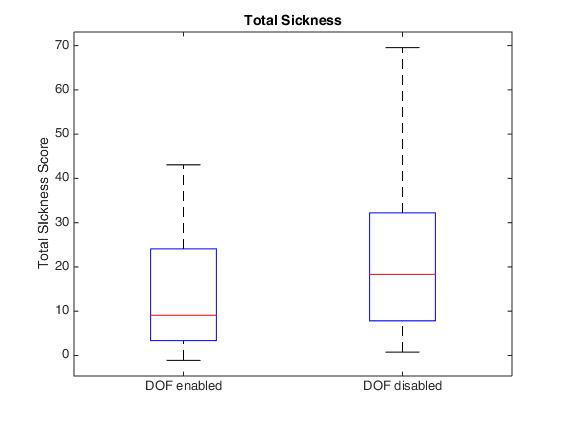
\includegraphics[width=0.5\textwidth]{images/total.jpg}
            \caption{Total sickness score for participants with (left) and without (right) DoF enabled.}
            \label{fig:totalSicknessScore}
\end{figure}


\begin{figure*}[t]
        \centering
            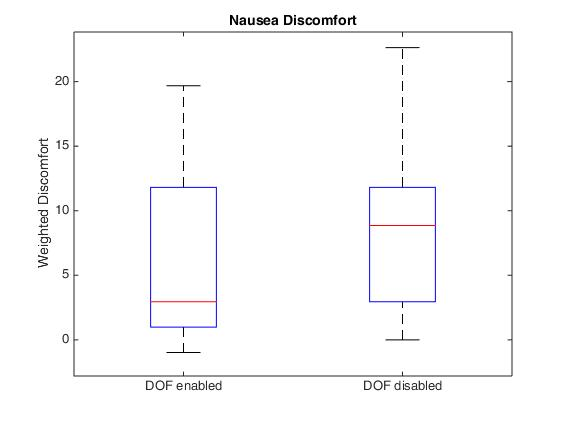
\includegraphics[width=0.32\textwidth]{images/nausea.jpg}
            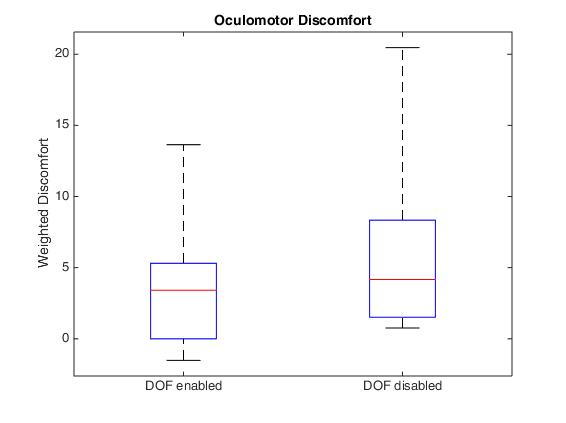
\includegraphics[width=0.32\textwidth]{images/oculomotor.jpg}
            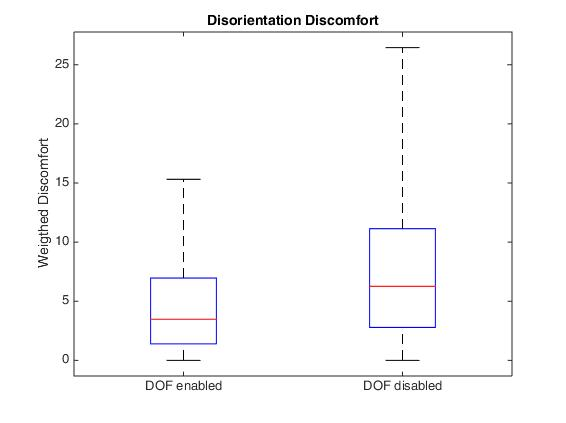
\includegraphics[width=0.32\textwidth]{images/disorientation.jpg}
            \caption{Change of sickness measure for each of the three discomfort categories: Nausea (left), Oculomotor (centre), Disorientation (right).}
            \label{fig:categorySickness}
\end{figure*}


Not all of the questions asked during our experiment were used to calculate sickness measures: anxiety and drowsiness responses were instead used to give a quantifiable estimation of a participant's mental state during the experiment. The loss of appetite and desire to move bowels results were also not used, as it was not feasible to control external factors such as time since the participant had last eaten, which were considered to significantly contribute to participant responses to these symptoms. \\

All of the participants who withdrew during our experiment did so in their first session, and every one of these sessions was one in which DoF blur was not enabled. Three of the withdrawals in the experiment occurred on unusually warm days; interior temperature was significantly higher than normal. The lab where this experiment was situated does not have an effective climate control system.\\

% moved to disucssion 
% There were a total of two participants who stated \say{(they) felt equally sick on both sessions}, and had consistent responses to their discomfort symptoms on each session. This indicates that there are people for whom DoF blur is not always relevant for reducing visual discomfort on HMDs: reducing the contribution of the accommodation-vergence conflict does not significantly affect overall their visual discomfort. 

% Possible reasons for this may include: these individuals were not well suited to the chosen HMD parameters (for example, they may have a IPD that differs significantly from the average), or they experienced an adverse reaction to a HMD factor that we did not explore which overpowered the contribution of the accommodation - vergence conflict to discomfort.
